\documentclass{sig-alternate}
%\documentclass{sig-alternate11pt1col}
\usepackage{verbatim}
\usepackage{algorithm,algorithmic}
\usepackage{enumerate}
\usepackage{mdwlist}
\usepackage[rgb]{xcolor}

\newcommand{\todo}{\color{blue}}

\usepackage{listings}
 \lstloadlanguages{% Check Dokumentation for further languages ...
         %[Visual]Basic
         %Pascal
         %C
         %C++
         %XML
         %HTML
         Java
 }

\begin{document}
% --- Author Metadata here ---
\conferenceinfo{SOCC'12,} {October 14-17, 2012, San Jose, CA USA} 
\CopyrightYear{2012}
\crdata{978-1-4503-1761-0/12/10}
\clubpenalty=10000
\widowpenalty = 10000
% --- End of Author Metadata ---

\title{All Aboard the Databus!}
\subtitle{Linkedin's Scalable Consistent Change Data Capture Platform}
%\subtitle{[Extended Abstract]}
%
% You need the command \numberofauthors to handle the 'placement
% and alignment' of the authors beneath the title.
%
% For aesthetic reasons, we recommend 'three authors at a time'
% i.e. three 'name/affiliation blocks' be placed beneath the title.
%
% NOTE: You are NOT restricted in how many 'rows' of
% "name/affiliations" may appear. We just ask that you restrict
% the number of 'columns' to three.
%
% Because of the available 'opening page real-estate'
% we ask you to refrain from putting more than six authors
% (two rows with three columns) beneath the article title.
% More than six makes the first-page appear very cluttered indeed.
%
% Use the \alignauthor commands to handle the names
% and affiliations for an 'aesthetic maximum' of six authors.
% Add names, affiliations, addresses for
% the seventh etc. author(s) as the argument for the
% \additionalauthors command.
% These 'additional authors' will be output/set for you
% without further effort on your part as the last section in
% the body of your article BEFORE References or any Appendices.

\def\sharedaffiliation{%
\end{tabular}
\begin{tabular}{c}}

\numberofauthors{1}
\author{
\alignauthor Shirshanka Das, Chavdar Botev, Kapil Surlaker, Bhaskar Ghosh\\
Balaji Varadarajan, Sunil Nagaraj, David Zhang, Lei Gao\\
Jemiah Westerman, Phanindra Ganti, Boris Shkolnik, Sajid Topiwala\\
Alexander Pachev, Naveen Somasundaram and Subbu Subramaniam\\
%
\sharedaffiliation
\affaddr{LinkedIn}\\
\affaddr{Mountain View, CA, USA}\\
\affaddr{\{sdas,cbotev,ksurlaker,bghosh,bvaradar,snagaraj,dzhang, lgao, jwesterman\}@linkedin.com}\\
\affaddr{\{pganti,bshkolnik,stopiwala,apachev,nsomasundaram,ssubramaniam\}@linkedin.com}
}
%\numberofauthors{15} %  in this sample file, there are a *total*
% of EIGHT authors. SIX appear on the 'first-page' (for formatting
% reasons) and the remaining two appear in the \additionalauthors section.
%
%\author{
% You can go ahead and credit any number of authors here,
% e.g. one 'row of three' or two rows (consisting of one row of three
% and a second row of one, two or three).
%
% The command \alignauthor (no curly braces needed) should
% precede each author name, affiliation/snail-mail address and
% e-mail address. Additionally, tag each line of
% affiliation/address with \affaddr, and tag the
% e-mail address with \email.
%
% 1st. author
%\alignauthor
%Shirshanka Das\\
%\email{sdas@linkedin.com}
%\alignauthor
%Chavdar Botev\\
%\email{cbotev@linkedin.com}
%\alignauthor
%Kapil Surlaker\\
%\email{ksurlaker@linkedin.com}
%\and
%\alignauthor
%Bhaskar Ghosh\\
%\email{bghosh@linkedin.com}
%\alignauthor
%Balaji Varadarajan\\
%\email{bvaradar@linkedin.com}
%\alignauthor
%Sunil Nagaraj\\
%\email{snagaraj@linkedin.com}
%}

%\additionalauthors{Additional authors: Phanindra Ganti (email: {\texttt{pganti@linkedin.com}}), Boris Shkolnik (email: {\texttt{bshkolnik@linkedin.com}}), David Zhang (email: {\texttt{dzhang@linkedin.com}})
%, Sajid Topiwala (email: {\texttt{stopiwala@linkedin.com}}), Alexander Pachev (email: {\texttt{apachev@linkedin.com}}), Lei Gao (email: {\texttt{lgao@linkedin.com}}), Jemiah Westerman (email: {\texttt{jwesterman@linkedin.com}})
%, Naveen Somasundaram (email: {\texttt{nsomasundaram@linkedin.com}}) and Subbu Subramaniam (email: {\texttt{ssubramaniam@linkedin.com}}).}

\maketitle
\begin{abstract}

In Internet architectures, data systems are typically categorized into source-of-truth systems that serve as primary stores for the user-generated writes, and derived data stores or indexes which serve reads and other complex queries.
The data in these query or index stores is often derived from the primary data through custom transformations, sometimes involving complex processing driven by business logic. Similarly data in caching tiers is derived from reads against the primary data store, but needs to get invalidated or refreshed when the primary data gets mutated. A necessary consequence of this kind of heterogeneous data architecture is the need to reliably capture, flow and process data changes happening in the primary data stores.

We have built Databus, a source-agnostic distributed change data capture system, which is an integral part of LinkedIn's data processing pipeline. The Databus transport layer provides latencies in the low milliseconds and handles throughput of thousands of events per second per server while supporting infinite lookback capabilities and rich subscription functionality. This paper covers the design and implementation and tradeoffs of the latest generation of Databus technology, experimental results from stress-testing the system and describes our experience supporting a wide range of LinkedIn production applications built on top of Databus.
\end{abstract}


\noindent
{\bf Categories and Subject Descriptors:} H.3.4 {[Systems and
    Software]}: {Distributed systems}

\noindent
{\bf General Terms:} Design, Algorithms, Replication, Change Data Capture, CDC, Stream Processing

%\category{C.2.4}{COMPUTER-COMMUNICATION NETWORKS}{Distributed Systems}{Distributed applications}
%\terms{Replication, Change Capture, Stream Processing}
\section{Introduction}

Scalable Internet architectures are typically composed of several specialized data systems. This is because web applications require a variety of data storage and query capabilities. Any single system is rarely a good fit to handle all the use-cases at scale while meeting the performance requirements. The most common data systems found in these architectures include relational databases, NoSQL data stores, caching engines and search indexes. Large scale social companies like LinkedIn will often build custom graph engines to handle complex graph queries at scale efficiently.

LinkedIn's data architecture consists of Oracle and MySQL as source-of-truth primary database technologies. There are a large number of specialized systems that have been built for serving complex use-cases like graph queries, search queries and ranking entities. Since reads outnumber writes by a large fraction in our workload, in many cases, we prefer to serve reads out of replica data stores; a technique commonly referred to as read-scaling. For example, there are cases when a single Oracle (running on expensive hardware) is the primary data store while many MySQL or Oracle instances (running on cheaper hardware) are serving reads. 
There are also other use-cases in the company that involve query result pre-computation, caching and near-line stream processing. 
There is therefore a need to capture all the changes that are happening to the primary databases and process it to populate the secondary data stores and indexes.
We also want to have a common data format that is both shared by all consumers and is independent of the source of truth. 
There are two ways we could have gone about building this. The first option is to write to the database and in parallel write to another messaging system. This is simple since the application code writing to the database is under our control. However it introduces a consistency problem because without a complex coordination protocol like Paxos~\cite{paxos} it is hard to ensure that both the database and the messaging system are in complete lock-step with each other in the face of failures. Both systems need to process exactly the same writes and need to serialize them in exactly the same order.
The second option is to make the database the source-of-truth, extract changes happening to the database and flow them through to the secondary data stores. This solves our consistency issue, but is challenging because databases like Oracle and MySQL have replication solutions that are proprietary. Since we want to process the data changes with application code and then write to secondary data stores, we need the replication system to be user-space and source-agnostic. This independence from the data source is especially important in growing companies, because it prevents technology lock-in and downstream consumers don't have to understand proprietary formats. 

After evaluating the pros and cons of the two approaches, we decided to pursue the second option in trying to achieve source-agnostic change data capture. 

%% Comments from Lin
%% The paragraph below needs a crisp list of strength/differentiators databus provides. Organize points in bullets will help.
%% Then we can have list of use cases, the longer, the more angels, the better.
  
We've built Databus which provides a common pipeline for transporting these change data capture (CDC) events from the primary databases to various applications. 
There are custom adaptors written for Oracle and MySQL which extract the changes happening in the database and convert them to a storage-neutral format. 
It is extremely easy to add support for other kinds of data sources as long as they provide a transaction log with some amount of rewindability.
These changes are then transported via a lossless tier while retaining the source consistency semantics to the final consumers. 
Databus allows consumers to fall behind indefinitely and still catchup while shielding the data source from abusive scan queries. 
The subscription API allows applications to subscribe to changes from one or more data sources, and filter based on the keys of the events.  
The Social Graph Index which serves all graph queries at LinkedIn, the People Search Index which powers all searches for members at LinkedIn and the various read replicas for our Member Profile data are all fed and kept consistent via Databus. 
\begin{figure}
\centering
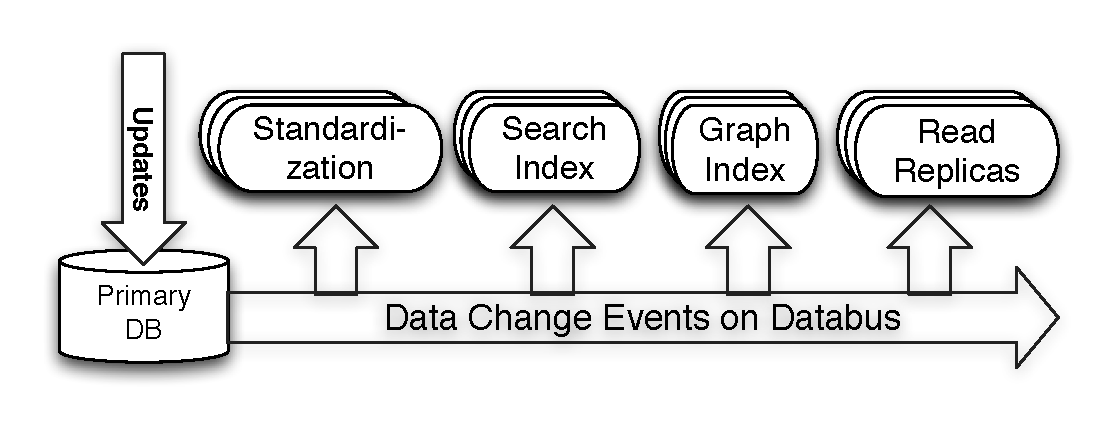
\epsfig{file=figures/databus-use-cases.eps, width=3in}
\caption{LinkedIn: Databus applications}
\label{fig:databus-use-cases}
\end{figure}






\section{Requirements}
We had the following requirements while designing Databus.
\begin{enumerate}[I]
\item \emph{No additional point of failure}: 
Since the data source is the source of truth, we want to ensure that the pipeline does not introduce a new point of failure in the architecture. 
\item \emph{Source consistency preservation}: 
We want to preserve the consistency semantics that the source provides. 
This implies needing to support the strongest consistency semantics possible. 
We do not support cross database transactions in the source. 
For transactional sources, to avoid having the subscribers see partial and/or inconsistent data we need to capture:
\begin{itemize}
\item \emph{Transaction boundaries}: a single user's action can trigger atomic updates to multiple rows across tables. 
\item \emph{Commit order}: the exact order in which operations happened on the primary database.
\item \emph{Consistent state}: we can miss changes but cannot provide a change-set that is not consistent at a point in the commit order. e.g. if a row got updated multiple times in quick succession, it is okay to miss an intermediate update, but not okay to miss the last update. 
\end{itemize}
\item \emph{User-space processing}: 
By ``user-space processing'', we refer to the ability to perform the computation triggered by the data change outside the database server. This is in contrast to traditional database triggers that are run in the database server.
Moving the computation to user space has the following benefits:
\begin{itemize}
\item Reduces the load on the database server
\item Avoids affecting the stability of the primary data store
\item Decouples the subscriber implementation from the specifics of the database server implementation
\item Enables independent scaling of the subscribers
\end{itemize}
\item \emph{No assumptions about consumer uptime}: 
Most of the time, consumers are caught up and processing at full speed. However, consumers can have hiccups due to variance in processing time or dependency on external systems, and downtime due to planned maintenance or failures. Sometimes, new consumers get added to increase capacity in the consumer cluster and need to get a recent snapshot of the database. In other cases, consumers might need to re-initialize their entire state by reprocessing the whole data set, e.g. if a key piece of the processing algorithm changes. Therefore, we need to support the capability to go back to an arbitrary point in time.
\item \emph{Isolation between Data-source and consumers}: 
Consumers often perform complex computations that may not allow a single instance to keep up with the data change rate. In those cases, a standard solution is to distribute the computation among multiple instances along some partitioning axis.
Therefore, the pipeline should
\begin{itemize}
\item Allow multiple subscribers to process the changes as a group; i.e. support partitioning;
\item Support different types of partitioning for computation tasks with different scalability requirements;
\item Isolate the source database from the number of subscribers so that increasing the number of the latter should not impact the performance of the former;
\item Isolate the source database from slow or failing subscribers that should not negatively impact the database performance;
\item Isolate subscribers from the operational aspects of the source database: database system choice, partitioning, schema evolution, etc.  
\end{itemize}
\item \emph{Low latency of the pipeline}: Any overhead introduced by the pipeline may introduce risk of inconsistencies, negatively affect performance, or decrease the available time for the asynchronous computations. For example, any latency in updating a secondary index structures (like the previously mentioned LinkedIn social graph index) increases the risk of serving stale or inconsistent data. In the case of replication for read scaling, pipeline latency can lead to higher front-end latencies since more traffic will go to the master for the freshest results. 
\item \emph{Scalable and Highly available}: We need to scale up to thousands of consumers and support thousands of transaction logs while being highly available. 
\end{enumerate}

\section{Architecture}

\begin{figure}
\centering
\epsfig{file=figures/databus-arch-v2.eps, width=3.2in}
\caption{Databus Architecture}
\label{fig:databus-architecture}
\end{figure}

The Databus architecture is split into four logical components. 
\begin{itemize}
\item a \emph{fetcher} which extracts changes from the data source or another Databus component, 
\item a \emph{log store} which caches this change stream, 
\item a \emph{snapshot store} which stores a moving snapshot of the stream, and 
\item a \emph{subscription client} which pulls change events seamlessly across the various components and surfaces them up to the application. 
\end{itemize}

The typical deployment architecture for these components is shown in Figure~\ref{fig:databus-architecture}. We collocate the fetcher and an in-memory log store in a process we call the \emph{relay} process. We additionally collocate a persistent log store and the snapshot store in a process we call the \emph{bootstrap service}. The subscription client is a library that is linked into the application that needs to consume changes from the stream. For a new type of data source technology (say PostgreSQL), the only component that needs to change in this architecture is the implementation of the db fetcher. 
 
\subsection{Consistency Semantics}
Databus supports transactional semantics across multiple types of entities within a transactional datastore. For example, it can annotate and propagate transactions that span multiple tables within the same database. It supports guaranteed at-least once delivery semantics by default. An event may be delivered multiple times only in the case of failures in the communication channel between the relay and the client, or in case of a hard failure in the consumer application. Consumers therefore need to be idempotent in the application of the delivered events or maintain transactional commit semantics aligned with the source. 

%The guarantee of lossless delivery is provided by the end-to-end pull architecture in Databus. Every failure can be recovered from by going up the chain and re-pulling from the checkpoint of the failure point. 


\subsection{External Clock and Pull Model}

The overarching design principle of Databus is that it is simply a lossless transporter of changes that have been committed upstream. Each change set is annotated with a monotonically increasing system change number~(SCN). This number is assigned by the data source and typically system specific. For example, Oracle attaches an SCN to each commit, while MySQL's commits can be identified uniquely through their offset in the binary log (binlog). As these changes flow through the ecosystem, derived state gets created by consumers and is associated back to the change stream through this number. This is important not just for auditing, but also to recover from failures and resume processing without missing any changes.  The system therefore is externally clocked. All parts of the Databus infrastructure track the lineage of data records and the progress of consumers using only the SCN of the external system. Physical offsets are only used as optimizations in internal transport but are never used as source of truth. 

There are many advantages of favoring pull over push in this particular context. We need to support a large number of consumers and allow them to consume from any arbitrary point in time. The most natural place to keep state of how much of the SCN timeline has been really processed is the consumer, because that is where the processing is taking place. Keeping state at the consumer naturally leads to a pull-based data transfer model. 
%The requirement to support change data consumption from an arbitrary point in the change timeline naturally leads to a pull data transfer model for consumers. 
The process can be entirely governed by the consumers; at any moment, they may decide to rollback to a previous point. 
Thus, all Databus components have to be stateless. 

Further, the requirements for not introducing new points of failures and source consistency preservation led us to adopt a pull data transfer model for the DB fetcher. In a hypothetical push-based model, failures in pushing the changes from the DB fetcher to the relay will either lead to aborted transactions (violating the first requirement) or changes that are lost by Databus (violating the second requirement). 

Figure~\ref{fig:pull-model} shows the interactions between the different fetcher components and the source clock across the relay, bootstrap log and snapshot store. In this example, the source has generated changes until SCN 102400, the relay has an in-memory buffer that covers all changes from 70000 to 100000, the bootstrap service's persistent log covers all changes from 30000 to 90000, and the bootstrap service's snapshot store covers all changes from 0 to 80000. Depending on where the consumer is currently at, it will pull from either the relay or the bootstrap service. 

\begin{figure}
\centering
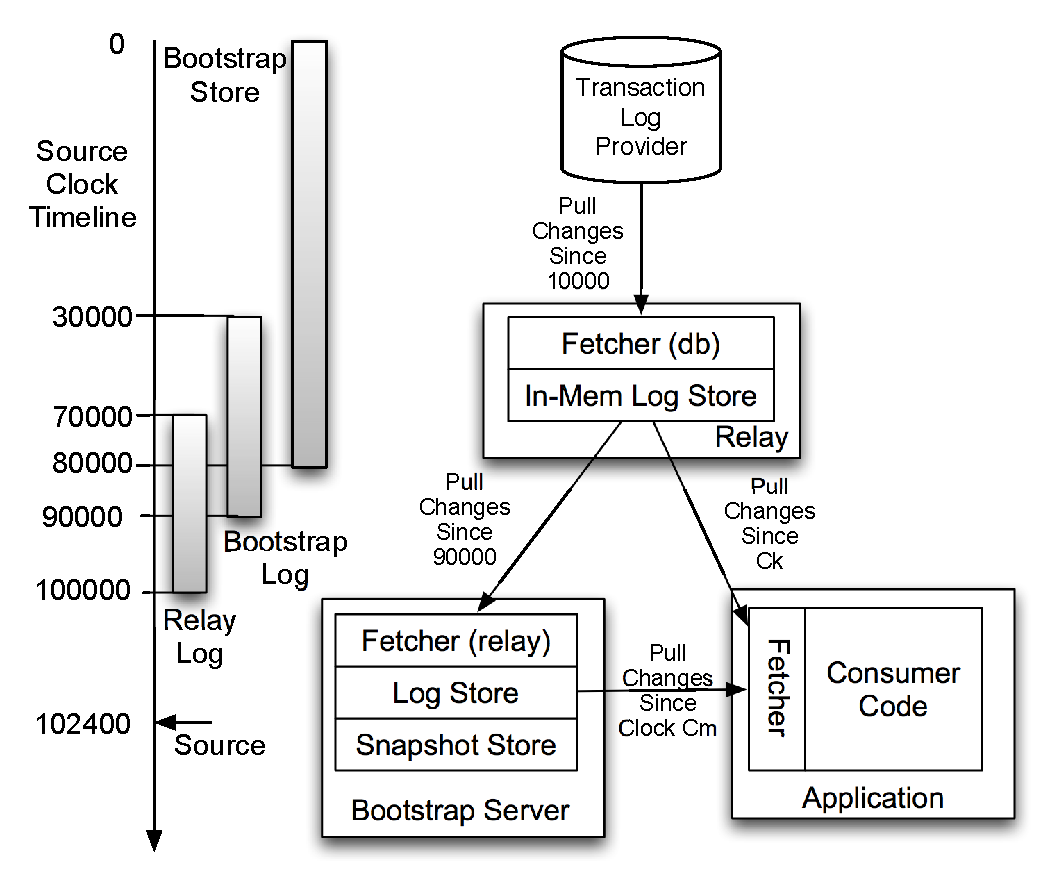
\epsfig{file=figures/databus-pull-model.eps, scale=0.50}
\caption{Pull Model and Source Clock}
\label{fig:pull-model}
\end{figure}

In addition to supporting simple restart and recovery semantics, this design also makes it very easy to integrate with non-Databus based data flows. 
%This is a very important design decision because it allows very simple restart and recovery semantics as well as integration with non-Databus based data flows. 
For example, an application can take a dump of an Oracle database, perform arbitrary processing on that dump, and then seamlessly tap into the Databus stream to get all changes that have happened to the database without missing a single change. The only requirement is that the original Oracle dump should be stamped with the same clock (Oracle's SCN system) that the Oracle Databus fetcher uses to pull changes out from Oracle. 

\subsection{Source Data Extract}
%The Fetcher: External Clock and Pull model}

Databus has been designed to support extraction from different data sources. This flexibility is achieved by allowing different fetchers to be developed and plugged into the pipeline. 
The fetcher is typically an embedded thread that gets run from within a relay and must follow a few semantic constraints.
As described above, each change set must be annotated with a monotonically increasing clock value that we refer to as the system change number~(SCN) of the change set.
This mapping from change set to SCN is immutable and assigned at commit time by the data source, therefore Databus can run multiple independent fetchers following the same timeline of changes without any need for synchronization. 
The fetcher is initialized with an SCN on startup, and must start pulling changes that are newer than this SCN from the data source. This in turn adds a ``rewindability'' requirement on the data source. 
The data source must be able to keep enough history in its change log or the fetcher must be written in a way that supports going back to pull from an arbitrary point in time. 
In practice, this requirement does not add any extra complexity on the source, but depending on the implementation, it can have a performance impact on the online writes that are happening on the data store. 
% as long as this lookback window is bounded (within a day or two). 
The way the Oracle fetcher is written, it can go back all the way to time zero, but since it queries the in-database tables, these queries get progressively expensive and impact the OLTP workload on the system. 
The MySQL fetcher mines the binary log directly, and can therefore rewind back to as much time as the storage on the MySQL machine will allow to retain without any performance penalty on the OLTP workload. 
We talk in detail about the implementation of these two fetchers in Section~\ref{sec:Implementation}.
Overall, this centralization of complexity onto the fetcher component leads to very simple persistence and failure-recovery protocols downstream. 
At the same time, fault-tolerance and high-availability in the relay tier and the presence of the snapshot store reduces the likelihood of having to go back in time on the data source, thus keeping the fetcher overhead low. 

%Extractors keep track of where they are in the timeline using checkpoints which typically contain a highwatermark corresponding to the contiguous section of the timeline that has been reliably processed so far. The fetcher is expected to be initialized with a checkpoint when it starts up or recovers from a failure. Once initialized, the fetcher keeps pulling changes from the data-source from that checkpoint onwards. As changes get processed, the fetcher keeps advancing the highwatermark and periodically stores the checkpoint in some persistence layer. This pure pull model ensures that the Databus transport layer is lossless. The only guarantees needed from the persistence layer is to not lose changes out of order. 

%Similarly, the only requirement this adds on the data source is that it should be able to support rewindable consumption; the fetcher can sometimes go back in time on failures. In most of the systems we've seen, this requirement does not add extra complexity on the source as long as this lookback window is bounded (within a day or two). The way the Oracle fetcher is written, it can go back all the way to time zero, but at the cost of queries that get progressively expensive. The MySQL fetcher can rewind back to as much time as the storage on the MySQL machine will allow to retain, without any performance penalties. This centralization of complexity onto the fetcher component leads to very simple persistence and failure-recovery protocols downstream.

\subsection{The Relay}
\label{sec:relay}
The Databus relay hosts a fetcher, a transient log and an HTTP server within a single process. 
As described earlier, the fetcher is a pluggable entity and can be used to fetch changes from a source or from another relay. 
The pluggability allows us to arrange relays in fan-out tree configurations for scaling out. 

The changes extracted by the fetcher are serialized into a binary format that is independent of the data source. They are then grouped together within transaction window boundaries, annotated with the clock value or SCN associated with the transaction and buffered in the transient log. These changes are handed out to consumers when they request them. The consumers request changes based on the source clock, asking for all changes since SCN \emph{N} where \emph{N} is the last SCN for which changes have been processed at the consumer. 

The relay does not maintain consumer-related state. Each consumer application progress is tracked through a consumer checkpoint maintained by the subscription client and passed on each pull request. Since all relays follow the same change stream timeline (determined by the commit order in the data source), the checkpoint is portable across relays.

On the one hand, the above simplifies the relay's implementation and the consumer fail-over from one relay to another. On the other hand, it causes an additional problem that the relay does not know if a given change set has been processed by all interested consumers. We therefore institute a time or size-based retention policy at the relay tier to age out old change sets. In practice, we provision the relays sufficiently using memory-mapped buffers to ensure that most consumers can consume the whole stream directly from the relay even while encountering minor hiccups, planned or unplanned downtime. The bootstrap service described in Section~\ref{subsec:Bootstrap} is the insurance policy in case of unforeseen downtime or if full data set reprocessing is required. We next describe the deployment models that are used in setting up relay clusters. 

\subsubsection{Relay Cluster Deployment}

Typical Databus deployments consist of a cluster of relay servers that pull change streams from multiple data sources. Each relay server can connect to multiple data source servers and host the change stream from each server in separate buffers in the same relay. The relays are also set up in such a way that the change stream from every data source is available in multiple relays, for fault-tolerance and for consumer scaling. There are two configurations the relays are typically deployed.

\begin{figure}
\centering
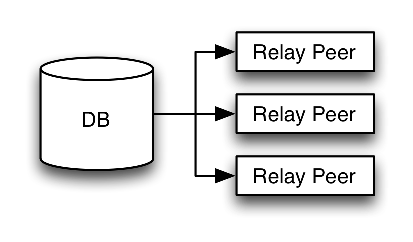
\epsfig{file=figures/relay_deployment_peers.eps, width=2.5in}
\caption{Independent Relay Deployment}
\label{fig:RelayDeployment1}
\end{figure}

In one deployment model as shown in Figure~\ref{fig:RelayDeployment1}, all the relay servers hosting a stream connect to the stream's data source directly. Each relay server is assigned a subset of all the streams being hosted by the relay cluster. The relay connects to the specified data source server and pulls the change streams. When a relay fails, the surviving relays continue pulling the change streams independent of the failed relay. If the configured redundancy factor is R, this model provides 100\% availability of the streams at very low latency as long as all the R relays that connect to the same data source server do not fail at the same time. This however comes as the cost of increased load on the data source server since there are R relays that pull the same change stream.

\begin{figure}
\centering
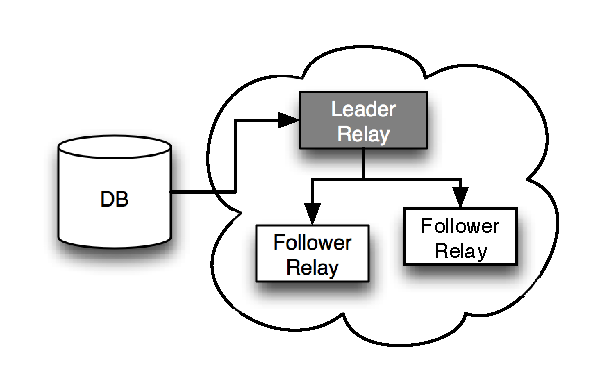
\epsfig{file=figures/relay_deployment_leader.eps, width=3in}
\caption{Leader-Follower Relay Deployment}
\label{fig:RelayDeployment2}
\end{figure}

To reduce the load on the source data source server, an alternative deployment model for relays as shown in Figure~\ref{fig:RelayDeployment2}, is the Leader-Follower model. In this model, for every data source server, one relay is designated to be the leader while R-1 are designated to be followers. The leader relay connects to the data source to pull the change stream while the follower relays pull the change stream from the leader. The clients can connect to any of the relays, either leader or follower. If the leader relay fails, one of the surviving followers is elected to be the new leader. The new leader connects to the data source server and continues pulling the change stream from the last sequence number it has. The followers disconnect from the failed leader and connect to the new leader. This deployment drastically reduces the load on the data source server but when the leader fails, there is a small delay while a new leader is elected. During this window, the latest changes in the change stream from the data source server are not available to the consumers.

To expand the capacity of the relay cluster, new relay servers can be added. When this happens, a new assignment of data source servers to relay servers is generated so that some streams are transferred from the old relay servers to the new relay servers. The new relay servers then connect to the data source servers and start pulling the change streams. They can optionally copy the existing change streams from the old relay servers before connecting to the data source servers.
This management of the relay cluster is built on top of a generic cluster management framework built at LinkedIn called Helix.

The assignment of data sources to relays is made available to Databus consumers in the form of a routing table so that the clients can discover the location of the streams they wish to consume. When the assignment changes due to relay failures or relay cluster rebalancing, this routing table is automatically updated and the consumers switch to the new servers transparently.





\subsection{The Bootstrap Service}
\label{subsec:Bootstrap}

As we have described previously, consumers typically subscribe to changes from the relay, which maintains an in-memory log store. Occasionally, there are situations in which the consumers might fall significantly behind in their processing. This usually happens because of consumer failures, which cause them to be offline for an extended period of time. In other cases, new consumers are launched and they need to bootstrap their initial state before consuming the change log from the relay. 

Possible approaches for dealing with these situations are going back to the source OLTP database and storing extended logs at the relays. The first approach is not acceptable since it leads to greatly increased load on the database that is serving online traffic. Besides, getting a consistent snapshot of all the rows in the OLTP database by running a long running query is very difficult. Storing the log at the relay for extended periods of time is not always viable since if the consumer has fallen behind a lot, consuming every change event is likely to be slow and unnecessary. It is much more efficient to catch up using a snapshot store which is a compacted representation of the changes i.e. only the latest state of every affected row needs to be consumed. 

Databus implements this functionality using a Bootstrap Service. As shown in Figure~\ref{fig:databus-architecture}, the bootstrap service consists of three components:
\begin{itemize*}
\item a \emph{bootstrap database}: This has two parts. One is a persistent log store that maintains the change log for an extended time. The other is a snapshot store of the data that represents a view of the database at a given point in time. 
\item a \emph{bootstrap producer}: This is really just a fetcher that subscribes to the change log from the relay and writes it to the log store in the bootstrap database. 
\item and a \emph{bootstrap applier}: This is just another fetcher that pulls from the log store and periodically merges the changes into the snapshot.
\end{itemize*}

%Splitting the responsibilities between the bootstrap producer and the bootstrap applier  has two advantages. First, it keeps the change log persistent over an extended period of time so that consumers that fall behind and do not find changes on the relay can catch up using the log in the bootstrap database. Second, it is able to handle long transactions on the source OLTP database easily since appending to the log is much cheaper than building the snapshot. This ensures that the bootstrap database has enough write throughput to keep up with the source. 

In the above design, the combination of both a snapshot store and a log store is what ensures the ability of the Bootstrap Service to provide consistent snapshots to the consumer applications from arbitrary points in the change stream. It is important to note that the snapshot store itself is not sufficient to achieve this goal as explained below.

Getting a consistent read of the snapshot by locking the snapshot store is not practical. For big data sets, it may take many hours for a consumer application to read and process the snapshot. If there are multiple consumers trying to bootstrap, the application of new changes to the snapshot store may be suspended indefinitely. Further, if the entire snapshot is read in one humongous batch, a small processing error may require restarting of the entire bootstrapping process. Instead, the Bootstrap Service needs to allow the consumer application to bootstrap the data in manageable batch sizes while new changes are applied to the snapshot store. Thus at the end of reading the snapshot, it may not be consistent -- the consumer application may have been observed some of the new changes while it may have missed others. To ensure consistency, the Bootstrap Service has to replay all the changes that have happened from the point when the snapshot read started. Thus, the need for a log store to buffer such changes.

Further, splitting the responsibilities between the relay fetcher and the log store fetcher ensures that the Bootstrap Service has enough write throughput to keep up with the data source: appending to the log store is much cheaper than building the snapshot store. Peaks in the write traffic are handled gracefully by letting the snapshot store lag slightly behind the newest changes.

The full bootstrapping algorithm with support for bootstrapping of multiple sources is described below.

%On the consumer side, when a consumer needs to bootstrap, it needs to obtain the change events from both the snapshot and log store so that the combination yields a consistent change set. This is complicated by the fact that the bootstrap producer is updating the snapshot simultaneously. Getting a consistent read of the snapshot by locking the snapshot is not efficient when it is large. Instead the consumer must constantly be allowed to make progress by pulling rows in manageable batch sizes while applier is merging changes from the log store. Since the snapshot data might change across batches, this results in an inconsistent read of the data during the time rows are being read from the snapshot store.  In order to guarantee consistent read at the end of the bootstrapping phase,  bootstrap service uses the following algorithm to deliver changes to the consumer.

\begin{algorithm}
\label{alg:bootstrap}
\caption{Bootstrap Consumption}{bootstrap}{($sources$)} 
\begin{algorithmic}
\STATE $startScn$ = current scn of the bootstrap db
\FOR{$i=0$ to $sources$.length}
\REQUIRE Source $S_{j}$ ($j < i$) is consistent as of $startScn$ \\
\COMMENT{Begin Snapshot phase}
\STATE Get all rows from $S_{i}$ where $rowScn < startScn$ \\
\COMMENT{Can be done in batches}
\STATE $targetScn$ = max SCN of rows in $S_{i}$
\COMMENT{Begin Catchup phase}
\FORALL{source $S$j such that $j \leq i$}
\STATE Get all rows from $S_{j}$ log store from startScn until targetScn
\ENDFOR
\STATE $startScn = targetScn$
\ENDFOR
\end{algorithmic}
\end{algorithm}

\subsection{Event Model and Consumer API}

\lstset{basicstyle=\small}


There are two versions of the consumer API, one that is callback driven and another that is iterator-based. 
At a high-level, there are eight main methods on the Databus callback API.
%%We show the callback based API at Listing~\ref{listing:DatabusConsumerAPI}.   
%%\begin{algorithm}
%%\lstset{caption={Databus Consumer API},label=listing:DatabusConsumerAPI}
%%\begin{lstlisting}
%%interface DatabusEventListener
%%{
%%  Result onStartDataEventSequence(SCN startScn);
%% Result onEndDataEventSequence(SCN endScn);
%% Result onStartSource(String source, 
%%                       Schema srcSchema);
%%  Result onEndSource(String source, 
%%                     Schema srcSchema);
%%  Result onDataEvent(DbusEvent e, 
%%                     DbusEventDecoder decoder);
%%  Result onCheckpoint(SCN checkpointScn);
%%  Result onRollback(SCN rollbackScn);
%%  Result onError(SCN rollbackScn);
%%}
%%\end{lstlisting}
%%\end{algorithm}

\begin{itemize*}
\item \emph{onStartDataEventSequence}: the start of a sequence of data events from an events consistency window.
\item \emph{onStartSource}: the start of data events from the same Databus source (e.g. Oracle table). 
\item \emph{onDataEvent}: a data change event for the current Databus source.
\item \emph{onEndSource}: the end of data change events from the same Databus source.
\item \emph{onEndDataEventSequence}: the end of a sequence of data events with the same SCN.
\item \emph{onCheckpoint}: a hint from the Databus client library that it wants to mark the point in the stream identified by the SCN as a recovery point
\item \emph{onRollback}: Databus has detected a recoverable error while processing the current event consistency window and it will rollback to the last successful checkpoint.
\item \emph{onError}: Databus has detected a unrecoverable error and it will stop processing the event stream.
\end{itemize*}.

The above callbacks denote the important points in the stream of Databus change events. A typical sequence of callbacks follows the pattern below.

\begin{verbatim}
onStartDataEventSequence(startSCN)
    onStartSource(Table1)
        onDataEvent(Table1.event1)
               ...
        onDataEvent(Table1.eventN) 
    onEndSource(Table1)
    onStartSource(Table2)
        onDataEvent(Table2.event1) 
              ...
        onDataEvent(Table2.eventM)
    onEndSource(Table2)
        ... 
onEndDataEventSequence(endSCN)
\end{verbatim}

Intuitively, the Databus client communicates with the consumer: "Here is the next batch of changes in the watched tables (sources). The changes are broken down by tables. Here are the changes in the first table, then the changes to the next table, etc. All the changes represent the delta from the previous consistent state of the database to the following consistent state."

The contract on all of the callbacks is that the processing code can return a result code denoting a successful processing of the callback, recoverable or unrecoverable error. Failures to process the callback within the allocated time budget or throwing an exception, results in a recoverable error.
In cases of recoverable errors, the client library will rollback to the last successful checkpoint and replay the callbacks from that point.

The offloading of state-keeping responsibility from the consumer simplifies the consumer recovery. The consumer or a newly spawned consumer can rewind back to the last known good checkpoint. For instance, if the consumer is stateful, they just need to tie the state that they are keeping with the checkpoint of the stream. On failure, the new consumer can read the state and the checkpoint associated with it and just start consuming from that point. If the stream consumption is idempotent, then the checkpoint can be maintained lazily as well. 


\subsection{Metadata} 
\begin{figure*}
\centering
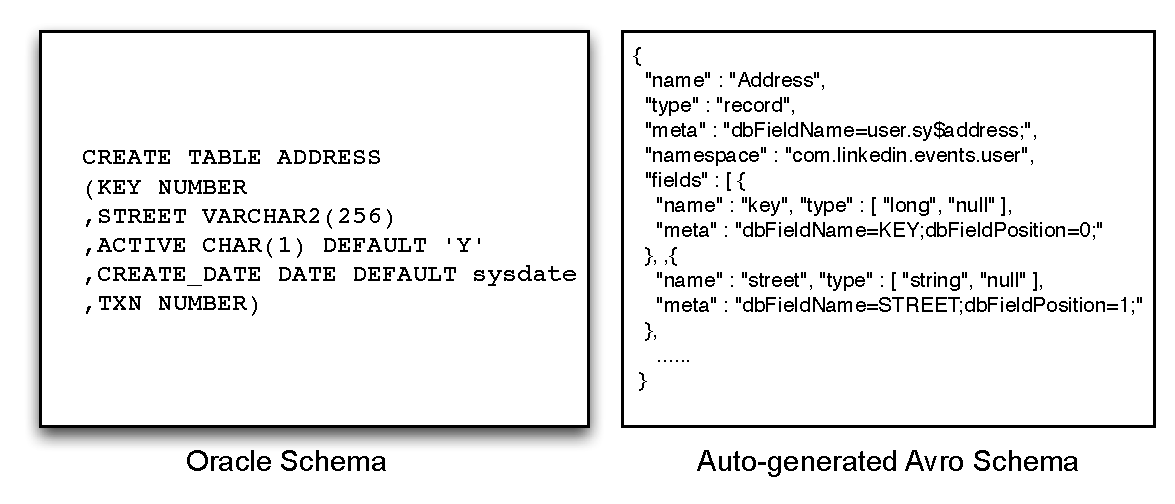
\epsfig{file=figures/oracle-avro-schema.eps, scale=0.75}
\caption{Oracle table mapped to Avro schema}
\label{fig:schema-mapping}
\end{figure*}

Databus uses Avro for serialization of events and supports schema versioning and evolution. This provides an isolation layer that protects consumers from upstream changes in the schema.

The fetchers infer the Avro schema by inspecting the source tables. Figure~\ref{fig:schema-mapping} shows a simple Oracle table mapped to an Avro schema. There are some intricacies when mapping data-types, e.g. when you have a column defined as NUMBER in Oracle, which one of int, long, float do you use when referring to the column in Avro? Once a schema is inferred, the relay is notified about it. When the fetcher generates new events from this table, it serializes the events with the Avro schema. When a table evolves, the schema for it changes and Databus attaches a newer version identifier to it. All new events are now serialized with this new schema version identifier. 

Databus ensures that changes to the source schema do not affect consumers and they can upgrade at their own cadence. The Databus client library performs automatic schema conversion using the standard  Avro schema resolution rules~\cite{avro} . We do not require reserialization of all older events generated since the beginning of time when the schema evolves because all versions of the schema are kept around forever. The schema resolution to an older version of the event schema is performed dynamically at the callback to the consumer. 

%\subsubsection{Relay Cluster Deployment}

Typical Databus deployments consist of a cluster of relay servers that pull change streams from multiple data sources. Each relay server can connect to multiple data source servers and host the change stream from each server in separate buffers in the same relay. The relays are also set up in such a way that the change stream from every data source is available in multiple relays, for fault-tolerance and for consumer scaling. There are two configurations the relays are typically deployed.

\begin{figure}
\centering
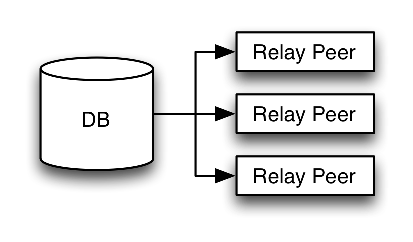
\epsfig{file=figures/relay_deployment_peers.eps, width=2.5in}
\caption{Independent Relay Deployment}
\label{fig:RelayDeployment1}
\end{figure}

In one deployment model as shown in Figure~\ref{fig:RelayDeployment1}, all the relay servers hosting a stream connect to the stream's data source directly. Each relay server is assigned a subset of all the streams being hosted by the relay cluster. The relay connects to the specified data source server and pulls the change streams. When a relay fails, the surviving relays continue pulling the change streams independent of the failed relay. If the configured redundancy factor is R, this model provides 100\% availability of the streams at very low latency as long as all the R relays that connect to the same data source server do not fail at the same time. This however comes as the cost of increased load on the data source server since there are R relays that pull the same change stream.

\begin{figure}
\centering
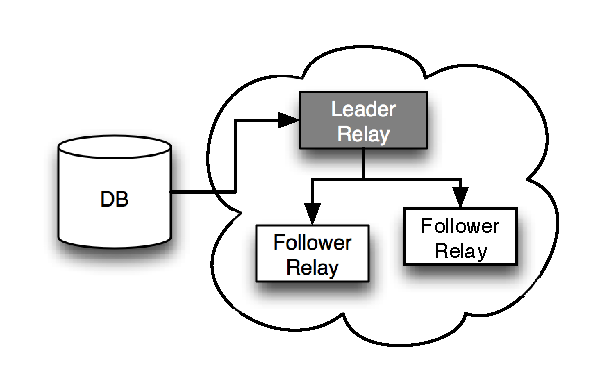
\epsfig{file=figures/relay_deployment_leader.eps, width=3in}
\caption{Leader-Follower Relay Deployment}
\label{fig:RelayDeployment2}
\end{figure}

To reduce the load on the source data source server, an alternative deployment model for relays as shown in Figure~\ref{fig:RelayDeployment2}, is the Leader-Follower model. In this model, for every data source server, one relay is designated to be the leader while R-1 are designated to be followers. The leader relay connects to the data source to pull the change stream while the follower relays pull the change stream from the leader. The clients can connect to any of the relays, either leader or follower. If the leader relay fails, one of the surviving followers is elected to be the new leader. The new leader connects to the data source server and continues pulling the change stream from the last sequence number it has. The followers disconnect from the failed leader and connect to the new leader. This deployment drastically reduces the load on the data source server but when the leader fails, there is a small delay while a new leader is elected. During this window, the latest changes in the change stream from the data source server are not available to the consumers.

To expand the capacity of the relay cluster, new relay servers can be added. When this happens, a new assignment of data source servers to relay servers is generated so that some streams are transferred from the old relay servers to the new relay servers. The new relay servers then connect to the data source servers and start pulling the change streams. They can optionally copy the existing change streams from the old relay servers before connecting to the data source servers.
This management of the relay cluster is built on top of a generic cluster management framework built at LinkedIn called Helix.

The assignment of data sources to relays is made available to Databus consumers in the form of a routing table so that the clients can discover the location of the streams they wish to consume. When the assignment changes due to relay failures or relay cluster rebalancing, this routing table is automatically updated and the consumers switch to the new servers transparently.



\section{Implementation Notes}
\subsection{Oracle Adapter}

Oracle provides replication support between Oracle databases using DataGuard. Additionally, there are commercial products like GoldenGate (from Oracle) that make the change log from Oracle available to external applications. In the absence of available open-source technology to solve this problem, a company has two options. It can either license the commercial solution with the associated fees and feature availability or try to develop and support its own solution. At the time LinkedIn was evaluating change capture technologies, GoldenGate lacked required features like BLOB/CLOB support. LinkedIn has implemented an Oracle change-capture mechanism based on triggers which we describe next.

A simple approach to get the change log from Oracle is to have a timestamp column with every row. A trigger on the table updates the timestamp column with the current time on an insert or update to the row as shown in Figure~\ref{fig:Tablewithtimestamp}. The adapter then issues a query to the database to get all the changed rows.

\begin{figure}
\centering
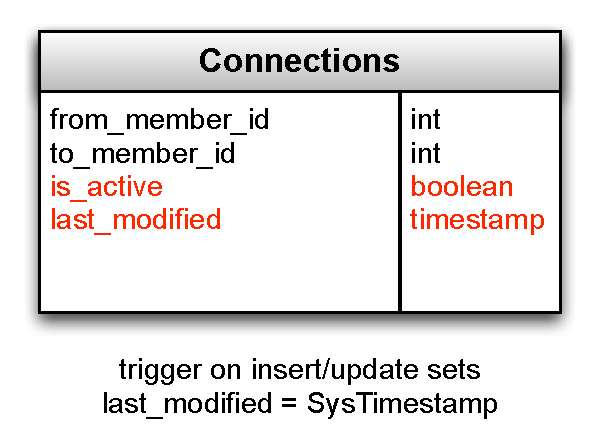
\epsfig{file=figures/timestamp-based-cdc.eps, scale=0.5}
\vspace*{-2ex}
\caption{Timestamp based CDC attempt}
\label{fig:Tablewithtimestamp}
\vspace*{-2ex}
\end{figure}

This however has a problem. Timestamps in this mechanism are set at the time of the change to the row, not at transaction commit. Long running transactions might have rows that changed long before the transaction finally commits. Thus, this query will miss changes from the database. For example in Figure~\ref{fig:tx1tx2}, tx2 commits before tx1 but t2 > t1. If the query happens between the two commits, lastTimeStamp is t2 and tx1 is missed. We can try some padding to reread rows that changed since $lastTimeStamp~-~n$ seconds but this is very error prone.

\begin{figure}
\centering
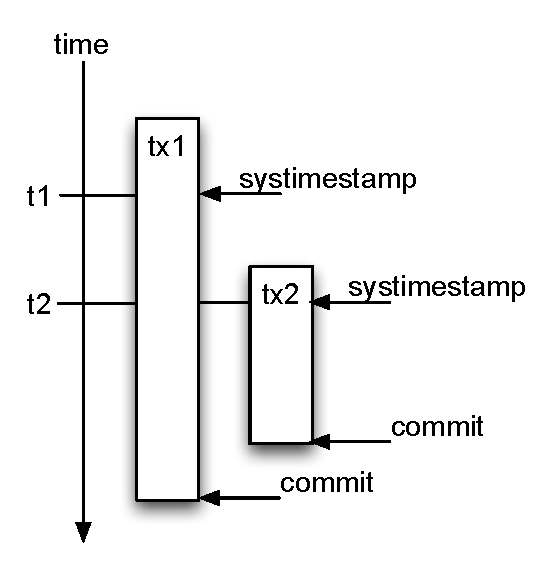
\epsfig{file=figures/timestamp-commit-reordering.eps, scale=0.50}
\vspace*{-2ex}
\caption{Timestamp based CDC: commit reordering}
\label{fig:tx1tx2}
\vspace*{-2ex}
\end{figure}
Oracle 10g and later versions provide a feature that provides the ora\_rowscn pseudo column which contains the internal Oracle clock (SCN - system change number) at transaction commit time. By default, ora\_rowscn is available at the block granularity but tables can be created with an option to provide ora\_rowscn at the row granularity. We can now query the database to fetch all rows that changed since the last rowscn but unfortunately ora\_rowscn is not an indexable column. To get around this problem, we add a regular column scn to the table and create an index on the column. The default value of scn is set to infinity. After commit, the ora\_rowscn for the affected rows is set. Every so often, we run a statement to update the scn column.

\begin{verbatim}
update T set scn = ora_rowscn
where scn = infinity;
\end{verbatim}

The query to select the changed rows since lastScn now becomes

\begin{verbatim}
select * from T 
where scn > lastScn 
AND ora_rowscn > lastScn;
\end{verbatim}

This works to get changes from a single table. However, transaction can span multiple tables in a database and these changes need to be transported to the consumer while preserving the transaction boundary. To solve this, we add a per database table TxLog that has the indexed scn column. We add a txn column to all the other tables that we wish to get changes from. We have a trigger than allocates txn from a sequence and adds an entry to the TxLog table on every transaction commit as shown in Figure~\ref{fig:txlog}. 

\begin{figure}
\centering
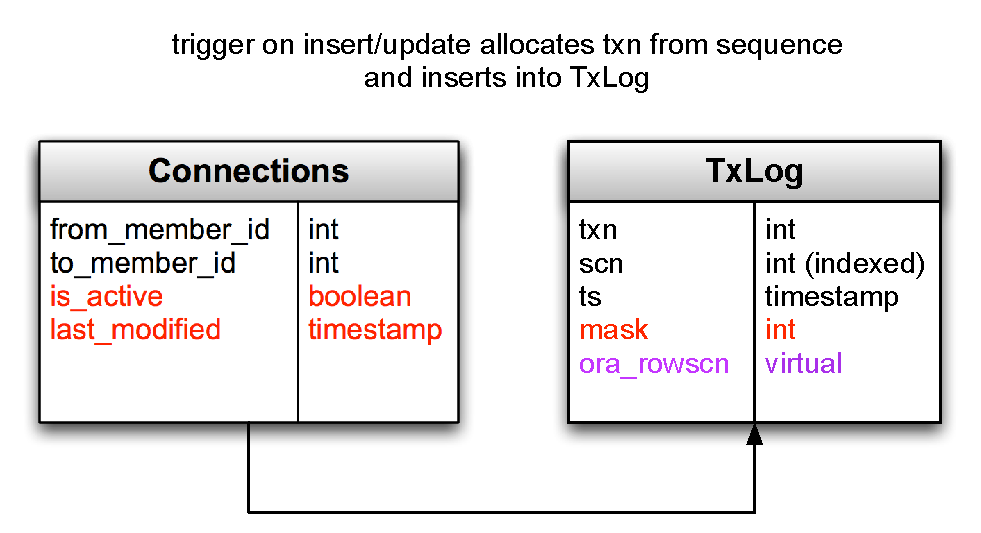
\epsfig{file=figures/txlog-based-cdc.eps, scale=0.50}
\vspace*{-2ex}
\caption{Trigger based CDC}
\label{fig:txlog}
\vspace*{-2ex}
\end{figure}

Changes can now be pulled using the following query

\begin{verbatim}
select src.* from T src, TxLog 
where scn > lastScn 
AND ora_rowscn > lastScn 
AND src.txn = TxLog.txn;
\end{verbatim}

The trigger-based approach used by the Oracle adapter has a couple of drawbacks. Firstly, it can miss intermediate changes to rows because it is only guaranteed to return the latest state of every changed row. This is not a correctness problem, but if possible, it is desirable to surface every change made to the row to the consumer.
Secondly, triggers and the associated tables that they update cause additional load in terms of reads and writes on the source database.



\subsection{MySQL Adapter}
The trigger-based approach used by the Oracle adapter has a couple of drawbacks. Firstly, it can miss intermediate changes to rows because it is only guaranteed to return the latest state of every changed row. This is not a correctness problem, but if possible, it is desirable to surface every change made to the row to the consumer.
Secondly, triggers and the associated tables that they update cause additional load in terms of reads and writes on the source database. 
It is more preferable to interact directly with the transaction log if that is possible, since that does not take up resources on the source database.
Oracle and MySQL both have binary logs which contain the log of changes as they are applied to the database. However, it is fragile to mine these logs and reverse-engineer the structure, because there is no guarantee that the format will be stable across multiple versions. In the case of MySQL though, it is possible to tap into the Storage Engine API which is a stable interface that has been used to build many commercial and open-source pluggable storage engines.

%The trigger based approach used by the Oracle Adapter guarantees that every poll issued to the database returns the latest state of every changed row. But it does not guarantee that every change made to that row in that duration is returned to the Adapter. In most cases, this is acceptable but in some usecases, it is desirable to make every change to the row available to the consumer. Another disadvantage of the trigger based approach is the additional load it puts on the source database. If the source database itself maintains a change log which can be read externally, that is a more efficient way for the adapter to pull the change log. In case of Oracle, the redo log is in a proprietary format and cannot be read externally unless Oracle's internal format is reverse engineered. MySQL on the other hand maintains a binary log of changes made to the database which is used by MySQL replication to replicate the changes between MySQL databases.

MySQL replication works only between MySQL databases and does not make the change log available to external applications. The pluggable storage engine layer allows MySQL replication to be setup between MySQL databases that might use different storage engines. 
%However, MySQL has a very elegant pluggable architecture that allows multiple storage engines to be plugged in using a common Storage Engine API. This feature of MySQL has created a thriving ecosystem of storage engines include MyISAM, InnoDB, PBXT, Tokutech etc. This feature allows MySQL replication to be setup between MySQL databases that might use different storage engines. 
Thus a MySQL server using InnoDB storage engine can replicate to MySQL server using the MyISAM storage engine. MySQL replication takes care of the protocol between master and slave, handling restarts across failures, parsing of the binary log and then calling the appropriate insert, update, delete statements on the slave through the storage engine API. Databus uses this feature of MySQL and obtains the change log from the MySQL master into a custom storage engine RPL\_DBUS which writes to the in-memory log. This architecture is shown in Figure~\ref{fig:mysql-adapter}. The relay manages the local slave MySQL instance and uses MySQL admin commands to connect to the MySQL master.

\begin{figure}
\centering
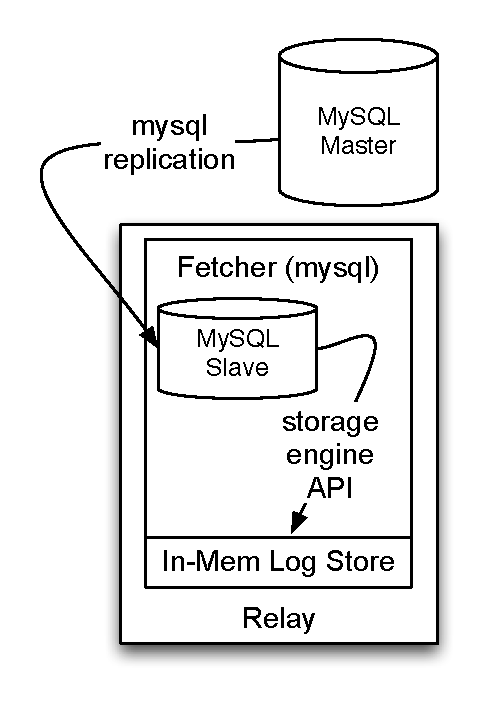
\epsfig{file=figures/mysql-adapter.eps, scale=0.4}
\caption{MySQL Adapter}
\label{fig:mysql-adapter}
\end{figure}

\subsection{Subscription Client Internals}
The Databus subscription client is the glue between the Databus infrastructure (relays, bootstrap service) 
and the Application (business logic in the consumer). 
The client is responsible for connecting to the appropriate relay and bootstrap service clusters, keeping track of progress in the Databus event stream, switching over automatically between the Relays and Bootstrap service when necessary, and performing conversions between the schema used for serialization of the payload and the schema expected by the consumer. 

The client runs a fetcher thread that is pulling continuously from the relay over a persistent HTTP connection and a dispatcher thread that fires callbacks into a pool of worker threads. There is local flow control between the fetcher and the dispatcher to ensure a steady stream of Databus events to the consumer. Two forms of multi-threaded processing are supported. The first type allows multi-threaded processing within a consistency window only. This ensures that consistency semantics are maintained at the destination. The second type allows multi-threaded processing without regard to the transaction window boundaries. This provides higher throughput at the consumer at the cost of relaxed consistency. 
The client maintains state of where it is in the sequence timeline through a customizable CheckpointPersister. By default, a checkpoint is persisted to disk for every successfully-processed consistency window. Applications that need very close control of the checkpoint may implement their own storage and restore for checkpoints to tie it to their processing state. For example, search indexes will often commit the checkpoint as meta-data along with the index files themselves so that they share the same fate. 



\section{Experiments}

In this section, we present our findings from a set of performance experiments that we ran to test the scalability characteristics of Databus. 

\subsection{Experimental setup}

We ran our experiments on two types of machines:

\begin{itemize}
\item Relays and client machines - 12 core 2.56GHz Intel Xeon machines with 48 GB RAM, 1TB SATA RAID 1+0 and 1 Gbps Ethernet
\item Bootstrap servers - 12 core 2.40GHz Intel Xeon machines with 48 GB RAM, 800GB 15K SAS RAID 1+0 and 1 Gbps Ethernet
\end{itemize}

There were three main parameters that we varied:

\begin{itemize}
\item Event rate - the rate at which change events are being fetched into the relay buffer
\item Number of consumers - the number of applications that consume events from the relays and bootstrap service
\item Consumer poll interval - the frequency with which consumers poll the relays for new events
\end{itemize}

For all experiments, we used moderately-sized events with a size of 2.5KB.

The metrics we measured were

\begin{itemize}
\item Throughput - the number of events or bytes per second that the relay can push out to the consumers
\item E2E event latency - the time it takes for an event to propagate from the relay to the consumers
\end{itemize}

\subsection{Relay}

Figure \ref{fig:relay_throughput} shows the first set of experiments where we measured the maximum relay throughput and CPU utilization with different sets of consumers. We used a relay with already pre-filled buffers and measured the maximum speed at which multiple consumers can read from the relay. We varied the number of consumers and the consumer poll interval. The latter parameter allowed us to test the impact of polling less frequently but in bigger batches of events. We expected that less frequent but bigger batches would allow the relay to support larger number of consumers. The data series prefixed with ``tpt'' show the relay throughput in MB/s (e.g. ``tpt\_10'' shows the throughput for consumers using 10ms poll interval) with throughput being plotted on the left-hand side ``y'' axis. The data series prefixed with ``cpu'' show the relay CPU utilization percentage (e.g. ``cpu\_55'' shows the throughput for consumers using 55 ms poll interval) with the CPU utilization being plotted on the right-hand side ``y'' axis.

\begin{figure}
\centering
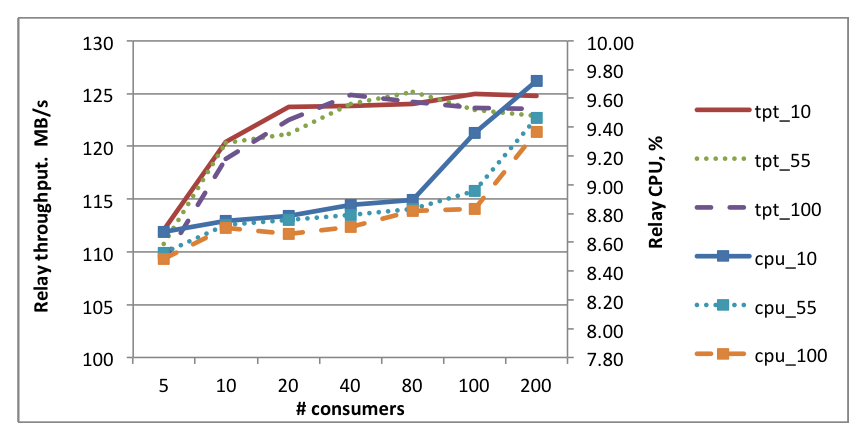
\epsfig{file=figures/relay_throughput.eps, width=3in}
\caption{Relay throughput scalability depending on poll interval}
\label{fig:relay_throughput}
\end{figure}

The experiments confirmed our hypothesis. With low poll intervals and fast processing consumers (as the ones that we used for our experiments), we can quickly saturate network bandwidth. We notice that once we get closer to network saturation, the relays do not scale linearly: doubling the number of consumers from 5 to 10 causes an increase of throughput of only 9\% (from 110MB/s to 120MB/s). We attribute this to networking overhead. The number of transmitted packets peaked at around 82 thousand packets/s even for 5 consumers and it did not increase with the number of consumers. Thus, increased number of consumers just leads to slightly better utilization of those packets.

Increasing the poll interval has only a small impact on the relay in terms of CPU utilization for small number of consumers. With increased number of consumers the effect becomes more pronounced although still the CPU utilization is fairly low -- less than 10\%. Overall, the experiments show that network bandwidth becomes a bottleneck much before the CPU. Thus, trading CPU for network bandwidth on the relay side can be expected to pay off. This is further explored in the experiments below.

The second set of experiments aimed at testing how writes to the relay buffer affected throughput. For this set of experiments, we gradually increased the update rate (100 update/s, 1000 updates/s, 2000 update/s) at the data source and measured the consumption throughput (in updates/s) and E2E latency (in milliseconds) at the consumers. Our goal was to detect when bottlenecks on the relay cause the consumers to fall behind the stream of updates from the data sources. We fixed the consumer poll interval at 10ms. Therefore, the consumers can expect on average 5 ms latency due to the poll frequency.   

Figure \ref{fig:throughput-poll10} shows the rate at which the consumers were receiving the events. For an event rate of 100 updates/s, the consumption rate stays flat at 100 updates/s, i.e. the consumers are keeping up with the update rate. For event rates of 1000 and 2000 updates/s, we observe two ``knees'' in the consumption rate when the number of consumers goes above 40 and 20 consumers respectively. These are the points at which the consumers are no longer able to keep up with the update stream. This behavior can again be explained by network bandwidth saturation: 40 consumers at 1000 updates/s utilize 100MB/s, close to the maximum network bandwidth. 

\begin{figure}
\centering
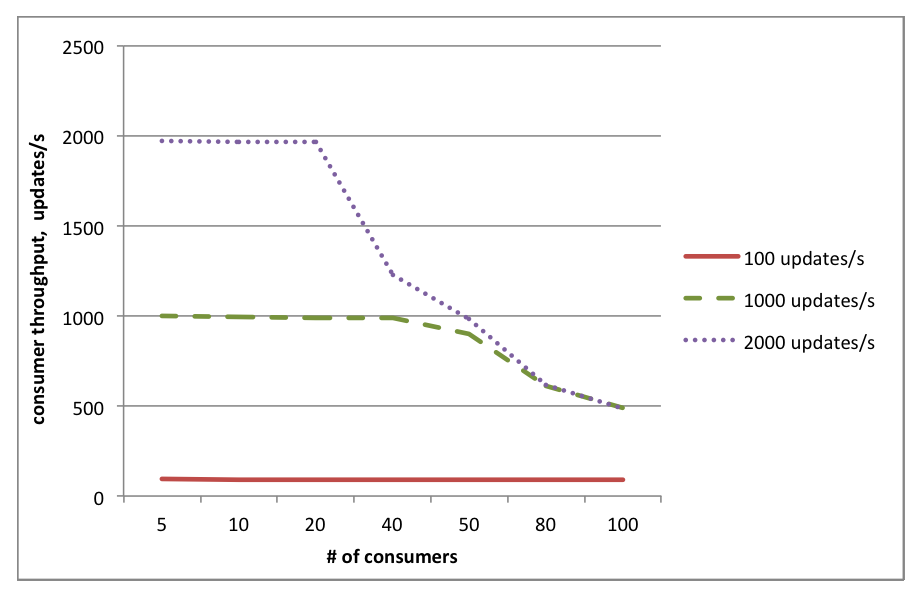
\epsfig{file=figures/consumer_throughput.eps, width=3in}
\caption{Throughput at consumers when varying update rate}
\label{fig:throughput-poll10}
\end{figure}

We observe a similar pattern when studying the E2E event latency on Figure~\ref{fig:latency-poll10}. At 100 updates/s, the E2E latency (including the poll interval) increases from 10ms to 20ms as the number of consumers grew. For 1000 and 2000 updates/s, we observe similar ``knees'' as the previous graph at 40 and 20 consumers. Up until those thresholds the E2E latency stays between 15 and 20ms and increases without recovery after that. 

\begin{figure}
\centering
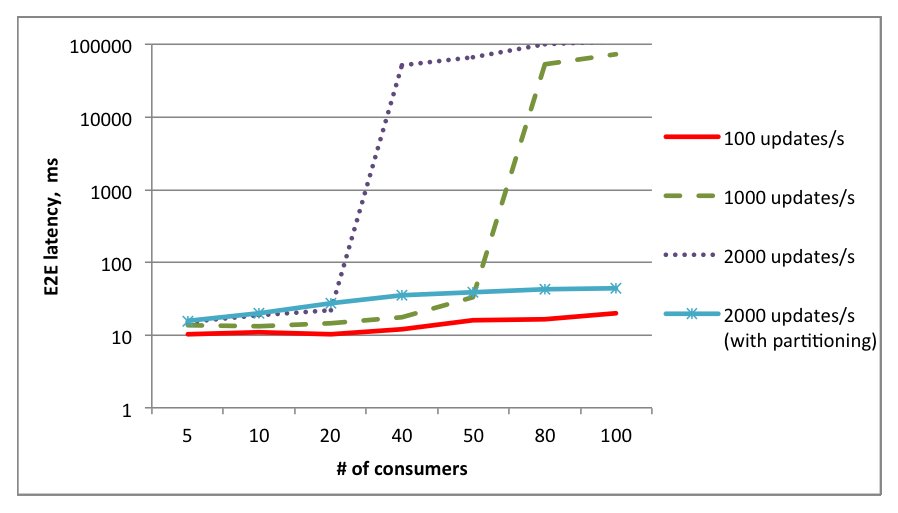
\epsfig{file=figures/e2e_latency.eps, width=3in}
\caption{Latency to consumers}
\label{fig:latency-poll10}
\end{figure}

For the experiment on Figure~\ref{fig:latency-poll10}, we also tested the effect of consumer partitioning using server-side filtering; each consumer only subscribes to a portion of the change stream. We wanted to remove the outbound network bandwidth bottleneck and see if the relay can scale to more consumers. The results are shown in the ``2000 updates/s (with partitioning)'' data series. For the experiment, we used a simple partitioning scheme where the key space is uniformly partitioned among all available consumers (a fairly typical scenario). In this case, the required outbound bandwidth is equal to the incoming data bandwidth and does not vary with the number of consumers. Although the E2E latency went up to a range of 15 to 45ms due to the additional server-side processing, the rate of increase in E2E latency is very gradual. Thus, we can conclude that the relay can scale to hundreds of consumers if the client application can tolerate slightly higher E2E latency.


\subsection{Bootstrap service}

We decided to setup our bootstrap performance experiments differently than our relay performance experiments. Firstly, the E2E latency metric used in the latter is not meaningful since the bootstrap service by definition serves older change records. Secondly, our initial bootstrap experiments showed that bootstrap servers can easily saturate the network bandwidth when bootstrapping multiple consumers, similarly to the relay experiments.

Instead, we focused on the more interesting aspect of the bootstrap service: the ability to serve compacted deltas of events from the snapshot store versus replaying all updates from the log store. 
On the one hand, serving from the log store utilizes very efficient sequential disk reads but has to return all change records. 
On the other hand, serving from the snapshot store allows the bootstrap service to stream out fewer records (because only the latest change record for a given key is returned) at the cost of a less efficient disk access pattern. 

The goal of our experiments was to find the break even point for the two access patterns. This helps us tune the retention policy in the bootstrap service and to implement an optimization in the bootstrap service where the snapshot phase can be bypassed if it is more beneficial to serve the bootstrap data entirely from the bootstrap log store. Thus, we introduced a new parameter: the ratio between updates to existing keys (including deletes) versus the total number of change records. This parameter models the benefit of returning only the latest version of the value for a given key. 

The experiments compared the time (in milliseconds) to do a full bootstrap on a set of test databases for which we varied the above ratio. We tested databases where the ratio varied from around 33\% to 99\%. The results are presented on Figure~\ref{fig:snapshot_vs_catchup}. 

\begin{figure}
\centering
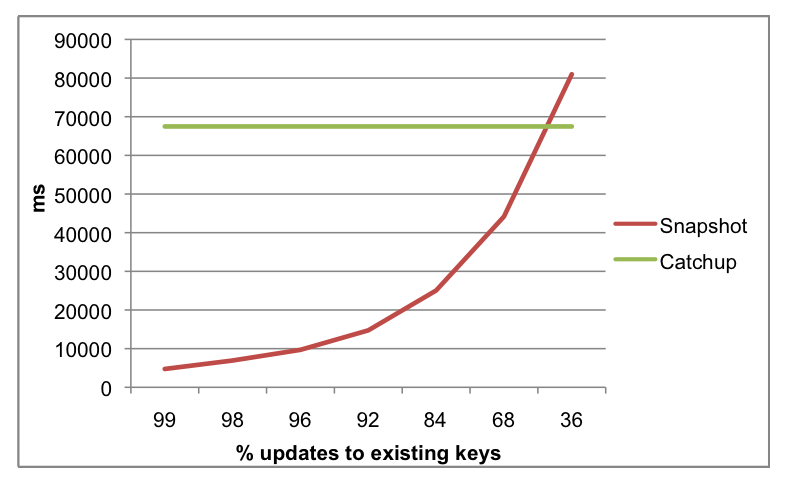
\epsfig{file=figures/snapshot_vs_catchup.eps, width=3in}
\caption{Time to bootstrap 1 hour of changes using a Snapshot delta or Catch-up log}
\label{fig:snapshot_vs_catchup}
\end{figure}

Our experiments show that with maintaining the appropriate index structures on the snapshot store, returning compacted deltas from the snapshot store is very efficient. The break-even point is when about half of the change records contain updates to existing keys. In practice, we actively monitor the above ratio in production and use the results from these experiments to tune our bootstrap services. Since the ratio changes slowly, the configuration is manual. In the future, we plan to make the bootstrap service auto-tunable.




\section{Experience in Production}
Databus has been in production at LinkedIn since its early days. It was originally developed to keep the graph engine in sync with the primary Oracle database.  
The original architecture~\cite{databus-qcon07} is shown in Figure~\ref{fig:databus-v1-arch}. It provided the consistency semantics that we needed and basic support for table-level subscription. The implementation included only relays and acted as a caching layer for the change stream from the database. Relays were constantly monitoring for new changes in the source database and buffering those in memory. If a consumer was lagging behind and its pull request could not be served from the in-memory buffer, the relay transparently created a proxied pull connection to the source database and fetched all changes needed by the consumer. 

With growth in traffic, number of consumers and the complexity of use cases, the original implementation started showing some scalability and operability limitations. This resulted in a significant redesign and rewrite of Databus. In this section, we look at how we fared and lessons learned from operating the system in the last two years. 

\begin{figure}
\centering
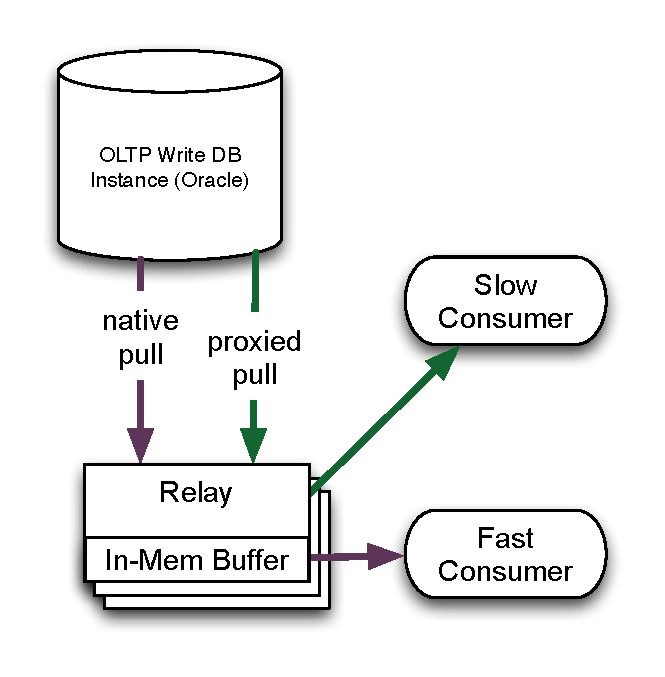
\epsfig{file=figures/databus-v1-arch.eps, scale=0.40}
\caption{LinkedIn: Databus Architecture circa 2007}
\label{fig:databus-v1-arch}
\end{figure}

\subsection{The Good}

\subsubsection{Source Isolation} 

In the original implementation of Databus, when a consumer fell too far behind, it would get proxied through to the source database. Our experience has shown that there are many reasons why clients often fall behind by a lot in unexpected ways. The most common cases happen when clients bootstrap themselves with state from data in offline systems like Hadoop, and then come online and have to catch-up a week's worth of data. Another set of cases arise due to software bugs. There have been cases where ``bad'' or unprocessable data has been written to the database or the consumer logic had bugs that made it choke on a particular event. Since the Databus framework provides in-order delivery guarantees, it retries some number of times and eventually pauses waiting for manual intervention. 
A third category of reasons are bursts or spikes of activity on the primary datasets. Downstream consumers which are typically provisioned for consuming the steady flow of events during normal operation, are unable to keep up with bursts of data and start falling behind. As explained in the Oracle fetcher implementation, the further the consumers fall behind, the more expensive the pull queries get. Thus, a problem on the consumer side gets translated to a problem on the source database. When we added the Bootstrap database to the Databus architecture, we took away the capability of the consumer to impact the source database in this way. Now, catch-up queries from consumers that are very far behind are served off of the bootstrap database that is isolated and optimized for this purpose. In this way, we've managed to reduce load on the source databases enormously while being able to keep up with the client demands easily.  We routinely see clients seamlessly connecting to the bootstrap service, sometimes on a daily basis but just catching up quietly without raising any alarm bells. 

\subsubsection{Common Data Format}

The original implementation of Databus used hand-written Java classes to represent the table rows, and serialized them using Java serialization. This created two problems. Firstly, every time the table's schema was changed, someone would have to hand-edit the Java class; secondly, because the Java serialization of that object was not backwards compatible with the previous version of the object, all downstream consumers would need to get upgraded to pick up the new class definition. The workaround for this problem was to create a new view every time the schema was changed, essentially creating one view per schema version on the database, and one copy of the event per version. As consumers evolved to picking up the new versions of the classes, the old views could be retired. In practice, consumers rarely had incentive to upgrade unless they needed the extra fields, thus the old views tended to stay around forever. The utilization of the relay buffer would worsen because each event would get serialized multiple times for each view version. In our latest changes, we moved to Avro, got rid of the multiple versions and this gave us an immediate three-fold performance win in terms of read and write load on the source database as well as utilization of the relay buffer. 

\subsubsection{Rich subscription support}

At LinkedIn we see a wide variety of consumers that are themselves partition-aware. For example, our distributed search system has many hundreds of nodes and each node only indexes a fraction of the complete data set. 
Often, different consumers want different partitioning functions or axes, and it is an organizational challenge to force everyone to agree to the same partitioning model. For example, our search engine
 uses range-based partitioning, while our relevance engine uses mod-based partitioning. Earlier, all the individual machines would pull the entire stream and filter it client-side by dropping the events that they were not interested in. When we added server-side filtering to Databus, we allowed consumers to specify their filtering function while subscribing to the sources. This has resulted in huge network savings which decreased the bandwidth requirements by 40 times.
\vspace{1in}
\subsection{The Bad}
We haven't solved all our problems yet. There are a few open challenges that we are working on addressing. 

\subsubsection{Oracle Fetcher performance}

Our experience has shown that several factors can negatively affect the performance of the Oracle fetcher:
\begin{enumerate*}
\item Databus sources in the form of complex join views are expensive because they have to be evaluated at fetch time.
\item Large BLOBs and CLOBs in rows can incur additional disk seeks.
\item The TxLog table grows over time which affects performance. Without time-based partitioning of the table, truncation of older rows requires maintenance with a period of write unavailability for the primary database.
\item Very high update rate can cause increased load on the SCN update job; this affects the effectiveness of the indexes on the TxLog table.
\item Very high write traffic can also lead to increased read and write contention on the TxLog table.
\end{enumerate*}

\subsubsection{Seeding the Bootstrap DB}

When launching Databus on existing tables, we have to go through the initial process of seeding the Bootstrap DB. This involves generating and loading a consistent snapshot of the source data. This can be a challenge for large data sets. Since stopping the writes to the primary store to seed the Bootstrap database is rarely an option, we either have to procure additional hardware to load a stable backup or devise an efficient restartable algorithm that can read the data out of the primary store in small chunks while guaranteeing that no updates are going to be missed and that all transactions that happen during the seeding process are fully applied at the end. We chose to use the second approach. Our production experience has shown that sources with complex joins and/or large BLOBs can negatively affect seeding performance. In some cases with complex joins, we have used dumps of the source tables and computed the joins offline (e.g. in Hadoop). With such an approach, the main challenge is ensuring that the offline join produces \emph{exactly} the same results as if it was performed by the primary store, because the two table dumps may not be consistent with each other.
%%\item \emph{Bottleneck identification}: Another class of experiences that we have had during our operation of Databus at LinkedIn is with identifying bottlenecks in the pipeline. The pervasiveness of the use of Databus at LinkedIn means that it is used in a large variety of scenarios with different types of consumer processing. Whenever a performance problem is observed, we need to detect whether it is because of bottlenecks in the Databus transport tier, inefficiencies in the way the application uses Databus or an external bottleneck such as a data store that the application is writing to. The last use case is typical for large consumer clusters where we can spend significant time optimizing performance to discover that the bottleneck is caused by scalability issues in another service used by the consumer.



\section{Related Work}

Change Data Capture (CDC) is not a new problem. However the environment in which it is required often determines the design trade-offs that get made in the architecture.
At LinkedIn, the expectations of paying customers and the requirement to offer a premium user experience motivated us to solve change capture in a scalable manner while not sacrificing data consistency or reliability. Related work in this area falls into two categories:
%Using a single shared data layer, e.g. sharded MySQL, usually works for online processing but data must still be made available to Data Warehouses and other offline processing systems such as Hadoop. One can also build on top of infrastructure such as GFS~\cite{gfs} that can be used for both online and offline use cases.
%Another common technique is to have the applications or mid-tier services do dual writes to the primary data layer as well a messaging system or write to a messaging layer first and then to the data layer~\cite{gizzard}. 
%Before we look at related work in this area, it is important to understand the context in which change data capture is implemented in Internet stacks. The common problem in this space is to make the changes to data in online databases available to various specialized systems. There are many different ways this problem gets solved, each with a different set of trade-offs.
%This works in situations where data loss and/or consistency problems are acceptable. LinkedIn has a large number of paying customers who demand high fidelity of their user data and a premium user experience. This requires that the data pipelines preserve consistency and avoid data loss.

\begin{itemize*}
\item \emph{Full featured CDC systems}: Many CDC systems such as Oracle DataGuard~\cite{dataguard} and MySQL replication~\cite{mysqlrepl} are restricted to replicating changes between specific source and destination systems. Other products such as Oracle Streams~\cite{streams} also make the change stream available through user APIs. Systems such as Golden Gate~\cite{goldengate} and Tungsten Replicator~\cite{tungsten} are capable of replicating from different sources to different destinations. But these are designed for usecases where the number of destinations is reasonably low and where consumers have a high uptime. In cases where consumer uptime cannot be guaranteed, seamless snapshotting and arbitrarily long catch-up queries must be supported. Most CDC systems are not designed for these scenarios.
 
%CDC systems are also designed to be either push-based or pull-based. In push-based systems, the source pushes changes to configured destinations. These are better suited for cases where low latency is desired but generally assume that destinations are reasonably low in number and largely available. Pull based systems on the other hand are better suited for consumers who may not be available at all times but have better support for batched consumption e.g. ETL into data warehouses. Our use cases require us to support both these use cases efficiently.
\item \emph{Generic messaging systems}
Messaging systems are sometimes used as transport to carry CDC data. There are some key trade-offs here. Messaging systems such as Kafka~\cite{kafka}, ActiveMQ~\cite{activemq} and other JMS implementations typically provide publish-subscribe APIs. Publishers are responsible for pushing changes to the messaging system, which is then responsible for guaranteeing the fate of the messages. Thus, the messaging system has to act as a \emph{source-of-truth} system. 
This leads to extra overhead for durability due to persistence, internal replication, etc. It also introduces potential for data loss in worst-case failure scenarios. In the presence of a reliable data source, this overhead is unnecessary.
%If reliability is a must, this puts extra burden on the system 
%If reliability is a must, the system has to go back to the publisher and ask for data if there is loss or corruption in the messaging system. 
\end{itemize*}


\section{Conclusion and Future Work}
In this paper, we've introduced Databus, LinkedIn's change data capture pipeline. 
Databus supports partitioned and non-partitioned transactional sources, very granular subscription capabilities and full re-processing of the entire data set while providing very low latencies and scaling to thousands of consumers with diverse consumption patterns. 
The interesting challenges we faced were mostly in the areas of:
\begin{itemize*}
\item Low-level systems design in building a low-latency high-throughput buffer that can scale to arbitrary size while supporting deep filtering on records.
\item Building an algorithm that can support consumers catching up from arbitrary points in time while maintaining a bounded amount of persistent state.
\item Layering the architecture in a way that is conducive to integration with a variety of data source technologies and amenable to flexible deployment strategies.
\end{itemize*}

Databus will be used as the internal replication technology for Espresso~\cite{linkedin12}, our distributed data platform solution. Databus will also provide external subscribers the capability to listen to the changes happening to the base dataset. We intend to explore some interesting avenues in the future. 
\begin{itemize*}
\item \emph{Relay-Client Protocol}: The current relay-client protocol is poll based. The client polls frequently to fetch new changes. With lots of clients polling frequently, this can lead to unnecessary resource utilization at the relay. We plan to add support for a streaming protocol, so that the client can make a request and just continue to read new changes off the response stream. This will lead to lower latencies as well as lower resource consumption. 
\item \emph{GoldenGate integration}: Recent releases of Oracle GoldenGate satisfy LinkedIn's requirements for CDC from Oracle. We are working on a Databus adapter that will pull changes from Oracle while avoiding the overhead of triggers. This change will not affect downstream consumers.
\item \emph{User defined processing}: The current subscription model allows consumers to pass in pre-defined filters for the changes that they are interested in consuming. We would like to extend that to support running user-defined processing on top of the stream. 
\item \emph{Change-capture for eventually consistent systems}: Our current implementation requires the source to provide a single transaction log or a set of partitioned transaction logs. Systems like Voldemort~\cite{linkedin12} do not fit into either category. It would be interesting to extend Databus to support such systems as data sources. 
\end{itemize*}

\section{Acknowledgments}

First and foremost, we would like to thank our shepherd Pat Helland who provided us with extremely insightful feedback for the final version of this paper. We would also like to thank the following people for their invaluable contributions to Databus: Jean-Luc Vaillant who is the spiritual father of Databus; 
Mitch Stuart and Yan Pujante who built and hardened the first version of Databus; 
our Operations partners Agila Devi, Jill Chen, Neil Pinto, Sai Sundar, Ramana Ramakrishnan, Nishant Vyas, Kevin Krawez, Brian Kozumplik and Zachary White; 
Lin Qiao, Tom Quiggle, Bob Schulman and Siddharth Anand who gave us continuous feedback during the preparation of this paper and last but not the least, all Databus customers at LinkedIn who've provided us with constructive feedback always.

\bibliographystyle{abbrv}
\small{\bibliography{sigproc}}
%\bibliography{sigproc}
\end{document}

